\documentclass[sutton_barto_notes.tex]{subfiles}
\begin{document}

\newpage
\textbf{Part II: Approximate Solution Methods}
In the second part, we are dealing with arbitrarily large state spaces; in these cases, it is hard to find $\pi_*$ or $v_*, q_*$.
Our goal instead is to find a good approximate solution using limited computational resources.

The problem with large state spaces is threefold: memory, time and data.
In many of our target tasks, almost every state encountered will never have been seen before. The solution is \textit{generalization}.
How can experience with a limited subset of the state space be usefully generalized to produce a good approximation over a much larger subset?

To some extent, we need only combine RL methods with existing  generalization methods. One of frequent use is \textit{function approximation}, which takes examples from a desired function (e.g. a value function) and attempts to generalize from them to construct an approximation of the entire function.

Function approximation is an instance of supervised learning.

RL with function approximation involves a number of new issues (usually not in SL), such as nonstationarity, bootstrapping, and delayed targets.

Chap 9 (prediction): on-policy training, policy is given and only its value function is approximated

Chap 10 (control): an approximation to the optimal policy is found

Chap 11: off-policy learning with function approximation

Chap 12: \textit{eligibility traces}, which dramatically improves the computational properties of multi-step RL methods in many cases.s

Chap 13 (control): \textit{policy-gradient}, a different approach to control, which approximates the optimal policy directly and need never form an approximate value function.

\newpage
\section{On-policy Prediction with Approximation}

We start consider using function approximation in estimating the state-value function from on-policy data, which approximates $v_\pi$ from experience generated using a known policy $\pi$.

The approximate value function is represented as a parameterized functional form with weight vector $\bm{w} \in \R^d$, instead of a table.
We write $\hat{v}(s,\bm{w}) \approx v_\pi(s)$ for the approximate value of state $s$ given weight vector $\bm{w}$.

For example,
\begin{itemize}
\item $\hat{v}$ = linear function in features of the state, $\bm{w}$ = vector of feature weights
\item $\hat{v}$ = function computed by a multi-layer ANN, $\bm{w}$ = vector of connection weights in all the layers
\item $\hat{v}$ = function computed by a decision tree, $\bm{w}$ = all the numbers defining the split points and leaf values of the tree
\end{itemize}

Typically, the number of weights is much less than the number of states ($d <<|S|$), and one weight takes care of many states.

Extending RL to function approximation also makes it applicable to partially observable problems (in which the full state is not available to the agent).

All theoretical results for methods using function approximation apply equally well to cases of partial observability.

Function approximation cannot augment the state representation with memories of past observations.

\subsection{Value-function Approximation}

\begin{definition}
\textbf{individual update notation}: $s \rightarrow u$ (the book uses $|->$, where $s$ is the state updated and $u$ is the update target. The estimated value for $s$ should be more like $u$.
\end{definition}

\begin{itemize}
\item MC: $S_t \rightarrow G_t$
\item TD(0): $S_t \rightarrow R_{t+1} + \gamma \hat{v}(S_{t+1},\bm{w}_t)$
\item n-step TD: $S_t \rightarrow G_{t:t+n}$
\item DP: $s \rightarrow \E_\pi [R_{t+1} + \gamma \hat{v}(S_{t+1}, \bm{w}_t) | S_t = s]$
\end{itemize}

We want to extend a one-to-one mapping to one-to-many mapping, i.e., updating $s$ will also update many other states.

Supervised learning methods learn to mimic input-output examples, and when the outputs are numbers, like $u$, the process is often called \textit{function approximation}.
We use these methods for value prediction simply by passing to them the $s \rightarrow u$ of each update as a training example.

In principle, we can use any method for supervised learning from examples, including ANN, decision trees, and various kinds of multivariate regression.
However, in RL, we require the methods are able to handle nonstationarity cases as RL agents need to do online learning (interact with the environment to obtain data).

\subsection{The Prediction Objective ($\overline{VE}$)}

By assumption we have far more states than weights, so making one state's estimate more accurate invariably(always) means making others' less accurate. We need to find which states we care most about.

\begin{definition}
\textbf{state distribution $\mu(s)$}: $\mu \geq 0$, $\sum_s \mu(s) = 1$, representing how much we care about the error (square distance between approx value $\hat{v}(s,\bm{w})$ and true value $v_\pi(s)$) in each state $s$.
\end{definition}

\begin{definition}
\textbf{Mean Squared Value Error ($\overline{VE}$)}: a natural objective function,
$$\overline{VE}(\bm{w}) \doteq \sum_{s\in S} \underbrace{\mu(s)}_{\text{weight}} \underbrace{[v_\pi(s) - \hat{v}(s,\bm{w})]^2}_{\text{error}}$$
\end{definition}

Often $\mu(s)$ is chosen to be the fraction of time spent in $s$. Under on-policy training, this is called \textit{on-policy distribution}. In continuing tasks, the on-policy distribution is the stationary distribution under $\pi$. The book talks about the episodic tasks (not including here).

!! NOTE that the RL community is not sure if $\overline{VE}$ is the right performance objective for RL. But this is the best we can find so far.

\subsection{Stochastic-gradient and Semi-gradient Methods}

In GD, the weight vector is a column vector with a fixed number of real valued components, $\bm{w} \doteq (w_1, w_2, ..., w_d)^T $, and the approximate value function $\hat{v}(s,\bm{w})$ is a differentiable function of $\bm{w}$ for all $s \in S$. However, no $\bm{w}$ can gets all the states in real world.

\paragraph{GD vs SGD} In both GD and SGD, we update a set of parameters in an iterative manner to minimize an error function.
\begin{itemize}
\item GD: we run through ALL the samples to do a single update for a parameter in a particular iteration (which is not feasible)
\item SGD: we run through ONLY ONE or a SUBSET of samples to do the update. If we use a SUBSET, it is called Minibatch Stochastic Gradient Descent.
\end{itemize}

The solution to $\bm{w}$ is SGD: we minimize error on the \textit{observed samples}. The weight vector of SGD is:
$$ \bm{w}_{t+1} \doteq \bm{w} - \frac{1}{2}\alpha \nabla [v_\pi(S_t) - \hat{v}(S_t, \bm{w}_t)]^2$$
$$ \bm{w}_{t+1} = \bm{w} + \alpha[v_\pi(S_t) - \hat{v}(S_t, \bm{w}_t)]\nabla \hat{v}(S_t, \bm{w}_t) $$

Now we consider when we do not have the exact true value $v_\pi(S_t)$, but an approximate value $U_t$. Then
$$ \bm{w}_{t+1} = \bm{w} + \alpha[U_t - \hat{v}(S_t, \bm{w}_t)]\nabla \hat{v}(S_t, \bm{w}_t) $$

If $U_t$ is an \textit{unbiased} estimate ($\E[U_t|S_t=s]=v_\pi(s)$), then $\bm{w}_t$ is guaranteed to converge to a local optimum under the usual stochastic approximation conditions (chap2). For example, Monte Carlo target $U_t\doteq G_t$ is an unbiased estimate of $v_\pi(S_t)$.

\begin{tcolorbox}[width=1.1\textwidth,title={Gradient Monte Carlo for Estimating $\hat{v}\approx v_\pi$}]
Input: $\pi$ to be evaluated, a differentiable function $\hat{v}:S\times\R^d \rightarrow \R$

Parameter: $\alpha > 0$

Init the value-function weights $\bm{w} \in \R^d$ arbitrarily

Loop forever (for each episode):

$\quad$Generate an episode $S_0, A_0, R_1, S_1, A_1, ..., R_T, S_T$ using $\pi$

$\quad$Loop for each step of episode, $t = 0,1,...,T-1$:

$\quad$Take action $A$; observe resultant reward, $R$, and state, $S'$

$\quad\quad$ $\bm{w} \leftarrow \bm{w} + \alpha [ G_t - \hat{v}(S_t, \bm{w})]\nabla \hat{v}(S_t, \bm{w})$
\end{tcolorbox}

On the other hand, Bootstrapping targets, such as $n$-step returns $G_{t:t+n}$ or the DP target, all depend on the current value of the weight vector $\bm{w}_t$, which implies that they will be biased. These are not the true gradient-descent methods, but $semi$-gradient methods.

Although semi-gradient (bootstrapping) methods do not converge as robustly as true gradient methods, they offer important advantages: (1) enable much faster learning; (2) enable learning to be continual and online; (3) provides computational advantages. A typical semi-gradient method is semi-gradient TD(0), which uses $U_t \doteq R_{t+1} + \gamma \hat{v}(S_t, \bm{w})$

\begin{tcolorbox}[width=1.1\textwidth,title={Semi-gradient TD(0) for Estimating $\hat{v}\approx v_\pi$}]
Input: $\pi$ to be evaluated, a differentiable function $\hat{v}:S\times\R^d \rightarrow \R$ where $\hat{v}(terminal,\dot)=0$

Parameter: $\alpha > 0$

Init the value-function weights $\bm{w} \in \R^d$ arbitrarily

Loop for each episode:

$\quad$Init $S$

$\quad$Loop for each step of episode:

$\quad\quad$Choose $A$~$\pi(\dot | S)$

$\quad\quad$Take action $A$; observe reward, $R$, and state, $S'$

$\quad\quad$ $\bm{w} \leftarrow \bm{w} + \alpha [ R + \gamma \hat{v}(S_t, \bm{w}) - \hat{v}(S,\bm{w})]\nabla \hat{v}(S_t, \bm{w})$

$\quad\quad S \leftarrow S'$

$\quad$until $S$ is terminal
\end{tcolorbox}

The target $U_t$ in semi-gradient methods is biased, so the $\bm{w}$ may not converge to a local optimum.



\paragraph{state aggregation} a simple form of generalizing function approximation in which states are grouped together, with one estimated value for each group.



\subsection{Linear Methods}

One of the most important special cases of function approximation is that, $\hat{v}(\dot, \bm{w})$ is a linear function of the weight vector $\bm{w}$. Corresponding to every state $s$, there is a real-valued vector $\bm{x}(s)\doteq (x_1(s),x_2(s),...,x_d(s))^T$, with the same number of components as $\bm{w}$.

Linear methods approximate the state-value function by the inner product between $\bm{w}$ and $\bm{x}(s)$:
$$\hat{v}(s,\bm{w}) \doteq \bm{w}^T\bm{x}(s)\doteq \sum_{i=1}^d w_i x_i(s) $$

The vector $\bm{x}(s)$ is a \textit{feature vector} representing state $s$. Each component $x_i(s)$ is a \textit{feature}.

The gradient of the approximation value function w.r.t $\bm{w}$ is then $\nabla\hat{v}(s,\bm{w})=\bm{x}(s)$.
Thus, we can simplify the general SGD update to
$$\bm{w}_{t+1} = \bm{w} + \alpha[U_t - \hat{v}(S_t, \bm{w}_t)]\bm{x}(s)$$

\paragraph{Understand the fixed point of linear TD learning}

Let us start with TD update with linear function approximation on the first line, recall the value of a state $\hat{v}(s,\bm{w}) \doteq \bm{w}^T\bm{x}(s)$
\begin{align*}
\bm{w}_{t+1} &\doteq \bm{w} + \alpha[R_{t+1} + \gamma\hat{v}(S_{t+1},\bm{w}_t) - \hat{v}(S_t, \bm{w}_t)]\bm{x}(S_t) \\
&= \bm{w} + \alpha[R_{t+1} + \gamma\hat{v}(S_{t+1},\bm{w}_t) - \hat{v}(S_t, \bm{w}_t)]\bm{x}_t \quad \text{simplify notation}\\
&= \bm{w} + \alpha[R_{t+1} + \gamma\bm{w}_t^T\bm{x}_{t+1} - \bm{w}_t^T\bm{x}_t]\bm{x}_t \quad \text{due to }\hat{v}(s,\bm{w}) \doteq \bm{w}^T\bm{x}(s)\\
&= \bm{w} + \alpha[\underbrace{R_{t+1}\bm{x}_t}_{\bm{b}} - \underbrace{\bm{x}_t(\bm{x}_t - \gamma\bm{x}_{t+1})^T}_{\bm{A}}\bm{w}_t] \quad\text{transpose doesn't change scalar}\\
\end{align*}
The TD update can be rewritten as the expected update + a noise term, so it is largely dominated by the behavior of the expected update.
\begin{align*}
\E[\Delta \bm{w}_t] &= \alpha(\bm{b} - \bm{A}\bm{w}_t) \\
\bm{b} &= \E[R_{t+1}\bm{x}_t] \\
\bm{A} &= \E[\bm{x}_t(\bm{x}_t - \gamma\bm{x}_{t+1})^T] \quad \text{expct. over features}
\end{align*}

\begin{definition}
\textbf{TD Fixed Point $\bm{w}_{TD}$}, the weight is converged when the expected TD update = 0.
$$\E[\Delta \bm{w}_{TD}] = \alpha(\bm{b} - \bm{A}\bm{w}_{TD}) = 0$$
\end{definition}
When $A$ is invertible, we can rewrite $\bm{w}_{TD} = \bm{A}^{-1}\bm{b}$. We say $\bm{w}_{TD}$ is a solution to this linear system; the solution is called TD fixed point.

$\bm{w}_{TD}$ minimizes an objective that is based on this $\bm{A}$ and $\bm{b}$. This objective extends the connection between TD and Bellman equations to the function approximation setting.

Recall in the tabular setting, TD is described as a sample based method for solving the Bellman equation. Linear TD similarly approximates the solution to the Bellman equation, minimizing what is called the projected Bellman error.

\paragraph{Describe a theoretical guarantee on the mean squared value error at the TD fixed point}

We want to understand the relationship between the solution found by TD and the minimum value error solution.
$$\overline{VE}(\bm{w}_{TD}) \leq \frac{1}{1-\gamma}min_{\bm{w}}\overline{VE}(\bm{w})$$
The difference between these two errors depends on $\gamma$ and the quality of features.

Why isn't the TD fixed point error equal to the minimum value error solution? This is because bootstrapping under function approximation. If our function approximator is good, then our estimate of the next state will be accurate.

\begin{tcolorbox}[width=1.1\textwidth,title={n-step semi-gradient TD for estimating $\hat{v}\approx v_\pi$}]
Input: $\pi$ to be evaluated, a differentiable function $\hat{v}:S\times\R^d \rightarrow \R$ where $\hat{v}(terminal,\dot)=0$

Parameter: $\alpha > 0$, $n > 0$

Init the value-function weights $\bm{w} \in \R^d$ arbitrarily

All store and access operations ($S_t$ and $R_t$) can their index mod $n+1$

Loop for each episode:

$\quad$Init and store $S_0 \neq$ terminal

$\quad T \leftarrow \inf$

$\quad$Loop for t = 0,1,2,...:

$\quad\quad$If $t<T$,then:

$\quad\quad\quad$Take an action according to $\pi(\cdot|S_t)$

$\quad\quad\quad$Observe and store $R_{t+1}$ and $S_{t+1}$

$\quad\quad\quad$If $S_{t+1}$ is terminal, then $T \leftarrow t+1$

$\quad\quad\tau \leftarrow t-n+1$ ($\tau$ is the time whose state's estimate is being updated)

$\quad\quad$If $\tau \geq 0$:

$\quad\quad\quad G \leftarrow \sum_{i=\tau + 1}^{min(\tau+n,T)} \gamma^{i-\tau-1}R_i$

$\quad\quad\quad$If $\tau + n < T$, then: $G\leftarrow G+\gamma^n \hat{v} (S_{\tau + n}, \bm{w})$

$\quad\quad\quad \bm{w} \leftarrow \bm{w} + \alpha [G - \hat{v}(S_{\tau},\bm{w})]\nabla \hat{v}(S_{\tau},\bm{w})$

$\quad$until $\tau = T-1$
\end{tcolorbox}

\subsection{Feature Construction for Linear Methods}

Choosing features appropriate to the task is an important way of adding \textit{prior domain knowledge} to reinforcement learning systems.

Linear methods,
\begin{itemize}
\item pro: guarantee convergence, data efficient, computation efficient
\item con: does not consider interactions between features
\end{itemize}

\subsubsection{Polynomials}
\subsubsection{Fourier Basis}
\subsubsection{Coarse Coding}

\begin{definition}
\textbf{binary feature}: 1-0 valued feature, 1 for present, 0 for absent.
\end{definition}
\begin{definition}
\textbf{coarse coding}: representing a state with binary features that overlap.
\end{definition}

\begin{figure}[h!]
  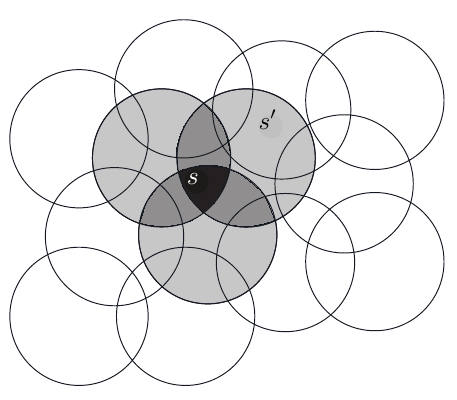
\includegraphics[width=0.7\linewidth]{c9-coarse-coding.png}
  \caption{Coarse coding. Generalization from $s$ to $s'$ depend on the number of their features whose receptive fields overlap}
  \label{fig:coarse-coding}
\end{figure}

\begin{figure}[h!]
  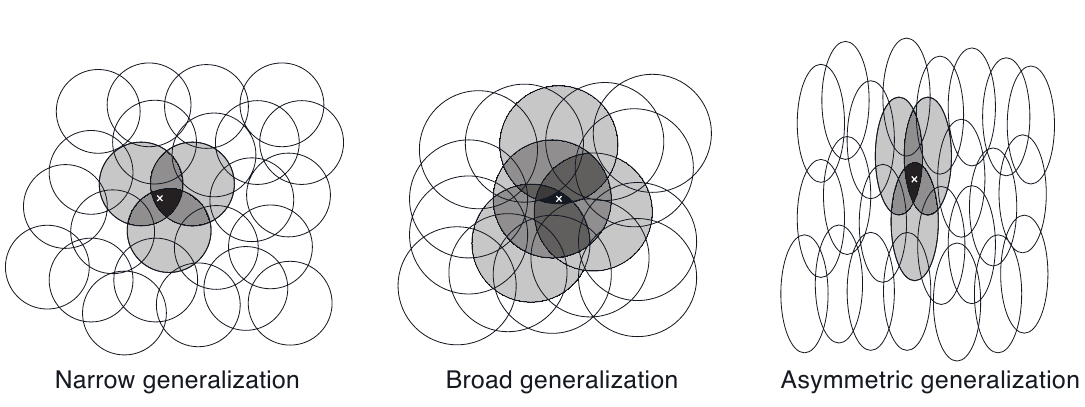
\includegraphics[width=0.7\linewidth]{c9-coarse-coding-2.png}
  \caption{Generalization in linear function approximation methods is determined by the sizes and shapes of the features' receptive fields. All three of these cases have roughly the same number and density of features.}
  \label{fig:coarse-coding}
\end{figure}

\subsubsection{Tile Coding}

\begin{definition}
\textbf{Tile coding}, a form of coarse coding for multi-dimensional continuous spaces that is flexible and computationally efficient.
\end{definition}
This may be the most practical feature representation for modern sequential digital computers.

In the coding, the receptive fields of the features are grouped into partitions of the state space. Each such partition is called a \textit{tiling}, and each element of the partition is called a \textit{tile}.

\subsection{Learning Objectives (UA RL MOOC)}

Lesson 1: Estimating Value Functions as Supervised Learning 

1. Understand how we can use parameterized functions to approximate value functions 

$\hat{v}(s, \bm{w})$

2. Explain the meaning of linear value function approximation 

$\hat{v}(s, \bm{w}) = \sum w_i x_i(s)$

3. Recognize that the tabular case is a special case of linear value function approximation. 

Consider each state has a corresponding vector (one-hot encoding)

4. Understand that there are many ways to parameterize an approximate value function 

ANN, decision tree etc

5. Understand what is meant by generalization and discrimination 

generalization: updates to the value estimate of one state influence the value of other states

discrimination:the ability to make the values for two states different to distinguish between the values for these two state.

6. Understand how generalization can be beneficial 

Generalization can speed up learning.

7. Explain why we want both generalization and discrimination from our function approximation 

Because we want generalization to speed up learning, and discrimination to distinguish really different states.

8. Understand how value estimation can be framed as a supervised learning problem 

Supervised learning involves approximating a function given a dataset of (input, target) pairs. For Monte-Carlo $(S_t, G_t)$. For TD $(S_t, R_t+\gamma\hat{v}(S_t, \bm{w}))$

9. Recognize not all function approximation methods are well suited for reinforcement learning 

Some are not suitable because they are designed for a fixed batch of data (offline learning, contrast to RL's online learning), or not designed for temporally correlated data (data in RL is always correlated).

Lesson 2: The Objective for On-policy Prediction 

10. Understand the mean-squared value error objective for policy evaluation 

We cannot guarantee perfect approximation for every state's value, so we need to define an objective, a measure of the distance between our approximation and the true values.
$$\overline{VE}(\bm{w}) \doteq \sum_{s\in\S} \underbrace{\mu(s)}_{\text{weight}} \underbrace{[v_\pi(s) - \hat{v}(s,\bm{w})]^2}_{\text{error}}$$

11. Explain the role of the state distribution in the objective 

$\mu(s)$ specifies how much we care for each state.
\begin{itemize}
\item It is a probability distribution
\item It has higher values for states that are visited more often
\item It serves as a weighting to minimize the error more in states that we care about
\end{itemize}

12. Understand the idea behind gradient descent and stochastic gradient descent 

We use SGD to optimize the objective $\overline{VE}$. (1) the gradient indicates the direction to increase/decrease the weight vectors; (2) the gradient gives the direction of steepest ascent

13. Outline the gradient Monte Carlo algorithm for value estimation 

see chap 9.3

14. Understand how state aggregation can be used to approximate the value function 

Group multiple states into one grouped state. One feature for each grouped state.

15. Apply Gradient Monte-Carlo with state aggregation 

see chap 9.3

Lesson 3: The Objective for TD 

16. Understand the TD-update for function approximation 

17. Highlight the advantages of TD compared to Monte-Carlo 

TD enables faster learning, continual and online learning; provides computational advantages

18. Outline the Semi-gradient TD(0) algorithm for value estimation 


see chap 9.3; semi-gradient TD as an approximation to SGD.

19. Understand that TD converges to a biased value estimate 

The TD target depends on our estimate of the value in the next state. This means our update could be biased because the estimate in our target may be inaccurate.

20. Understand that TD converges much faster than Gradient Monte Carlo 

TD can learn during the episode and has a lower variance update.

Lesson 4: Linear TD 

21. Derive the TD-update with linear function approximation 
$$\bm{w}_{t+1} = \bm{w} + \alpha[U_t - \hat{v}(S_t, \bm{w}_t)]\bm{x}(s)$$

22. Understand that tabular TD(0) is a special case of linear semi-gradient TD(0)

linear TD is a strict generalization on both tabular TD and TD with state aggregation. Recall the feature vector is like one-hot encoded vector, where the i-th=1, else 0 corresponds to i-th weight. 

23. Highlight the advantages of linear value function approximation over nonlinear 

\begin{itemize}
\item linear methods are simpler to understand and analyze mathematically
\item with good features, linear methods can learn quickly and achieve good prediction accuracy
\end{itemize}

linear semi-gradient TD (aka TD with linear function approximation)

-----------------------------------------

Lesson 1: Feature Construction for Linear Methods 

24. Describe the difference between coarse coding and tabular representations 

25. Explain the trade-off when designing representations between discrimination and generalization 

26. Understand how different coarse coding schemes affect the functions that can be represented 

27. Explain how tile coding is a (computationally?) convenient case of coarse coding 

28. Describe how designing the tilings affects the resultant representation 

29. Understand that tile coding is a computationally efficient implementation of coarse coding 

Lesson 2: Neural Networks 

30. Define a neural network

31. Define activation functions

32. Define a feed-forward architecture 

33. Understand how neural networks are doing feature construction 

34. Understand how neural networks are a non-linear function of state 

35. Understand how deep networks are a composition of layers 

36. Understand the trade-off between learning capacity and challenges presented by deeper networks 

Lesson 3: Training Neural Networks 

37. Compute the gradient of a single hidden layer neural network 

38. Understand how to compute the gradient for arbitrarily deep networks 

39. Understand the importance of initialization for neural networks 

40. Describe strategies for initializing neural networks 

41. Describe optimization techniques for training neural networks

\end{document}